
\subsection*{Recursieve backtrack algoritme}

In onze experimenten met ons eigen recursieve backtracking algoritme in \textsc{Matlab} bleek het algoritme perfect te werken voor NL4--10, degelijk voor NL12, en slecht voor NL14--16. 

Uit nader onderzoek blijkt dit te komen door het aantal backtracks; voorlopig wordt echter gewoon het algoritme in deze vorm gebruikt. 
De resultaten met het recursieve backtrack algoritme om initi\"ele schedules te maken, zijn samengevat in tabel~\ref{tab:random}.


 \begin{table}[hbpt]
 \centering 
 \begin{tabular}{c S S S S }\toprule
$n$ & {min (s)} & {avg (s)} & {max (s)} & {std (s)}  \\\midrule
 4   & 0.004	& 0.006	& 0.009	& 0.002 \\
 6   & 0.011&	0.017&	0.044&	0.010\\
 8  &  0.020	&1.889	&18.558&	5.857  \\
 10  & 0.031	&14.271	&112.291&	35.549\\
 12 &0.055	&8.795	&51.114&	16.583 \\
 14 & 0.089	&96.782	&612.953&	195.414\\
 16  &  1.088&286.021	&823.226	&360.467 \\
 \bottomrule
 
 \end{tabular}
\caption{Tijd nodig om een random schedule te maken via een recursief backtrack algoritme ($N=10$). \label{tab:random}}
 
 \end{table}

\subsection*{TTSA}
Wegens tijdsrestricties werden niet voor elke instantie even veel experimenten uitgevoerd. 
De experimenten werden ook niet slechts op een enkele computer uitgevoerd en ook niet onder dezelfde omstandigheden, dus de tijdaanduidingen geven slechts een grootteorde weer.

Eerst werden de parameters uit de paper geprobeerd. Deze gaven echter redelijk teleurstellende resultaten: het duurde namelijk enorm lang om oplossingen te vinden met kwaliteit vergelijkbaar zoals in de paper. De fast cooling schedules werkten echter behoorlijk: deze werden dan ook het meest getest. Figuren~\ref{fig:ttsafc6vs} en \ref{fig:ttsafc6} tonen dit voor NL6.
\begin{figure}[hbpt]
\centering
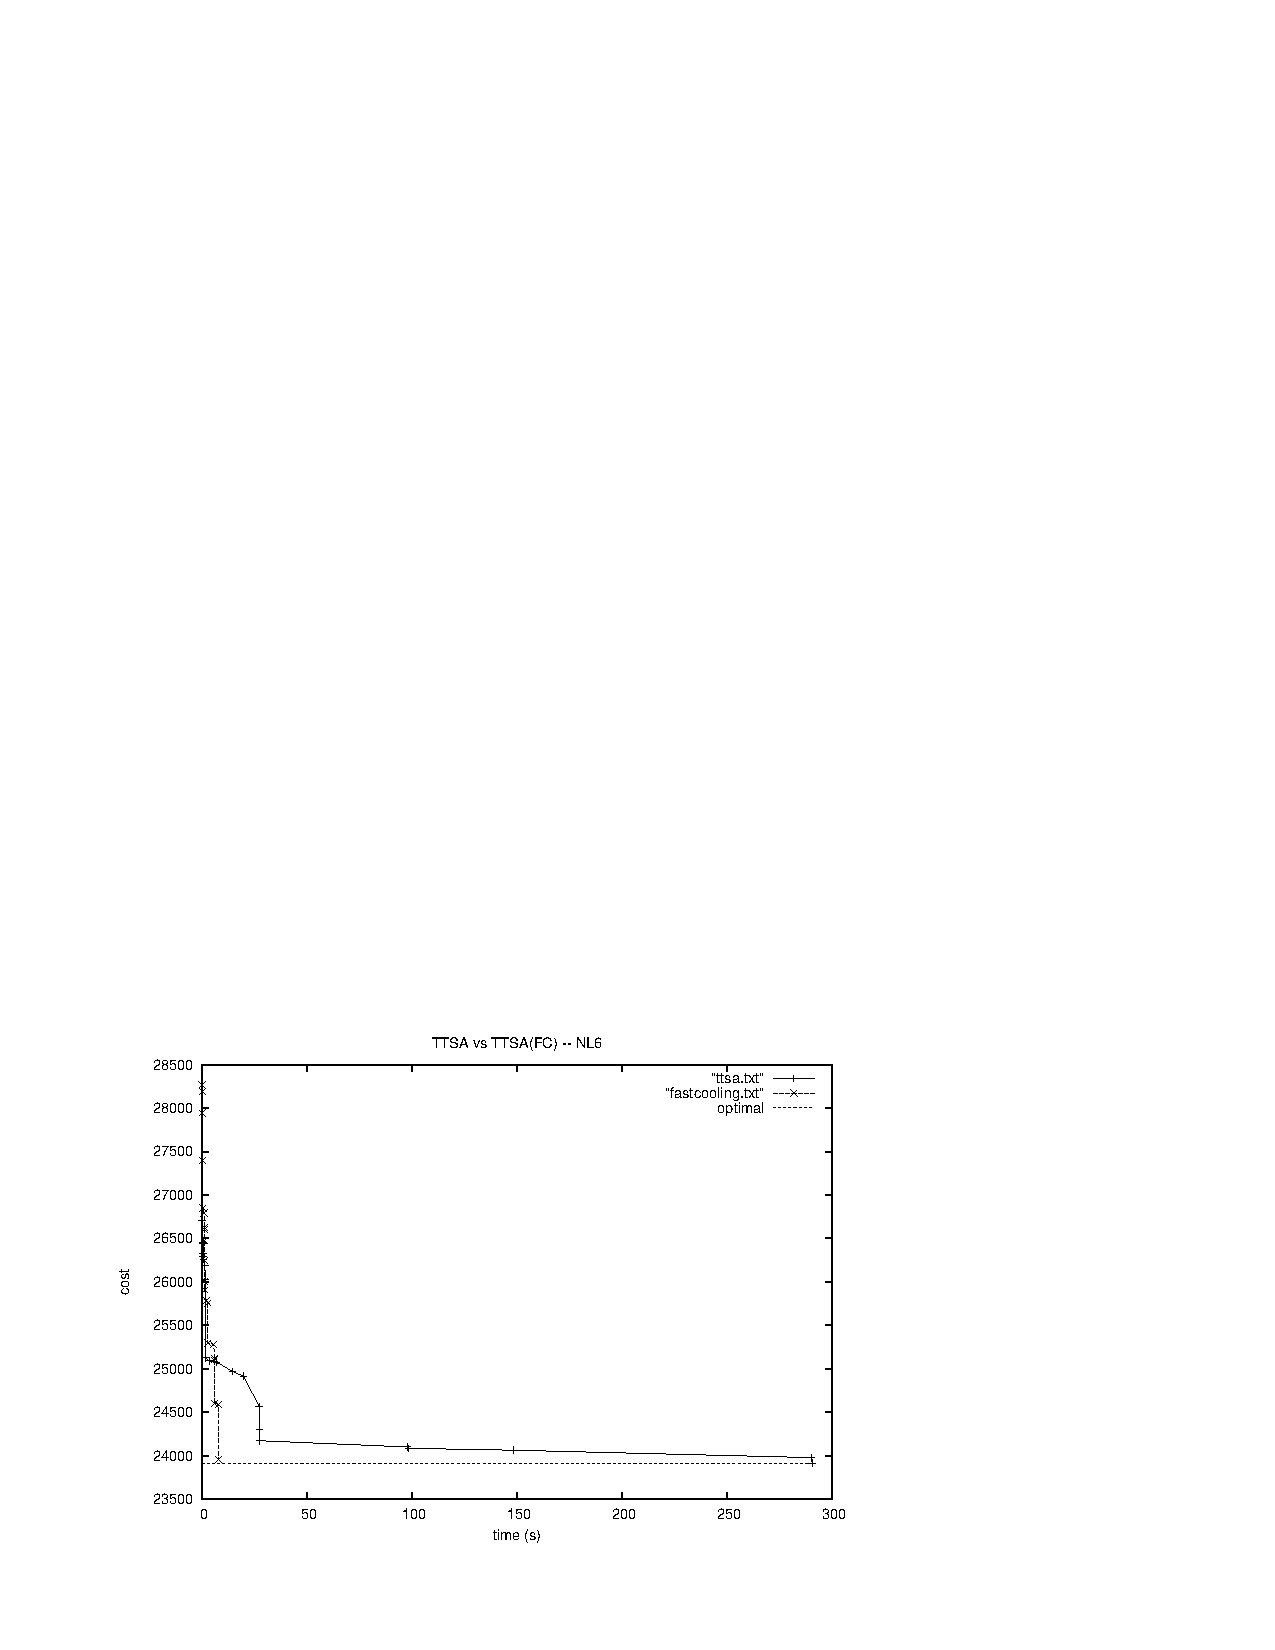
\includegraphics[width=0.75\textwidth,keepaspectratio=true]{nl6_ttsaVSttsaFC}
 \caption{TTSA vs TTSA(FC) NL6.}
 \label{fig:ttsafc6vs}
 \end{figure}

\begin{figure}[hbpt]
\centering
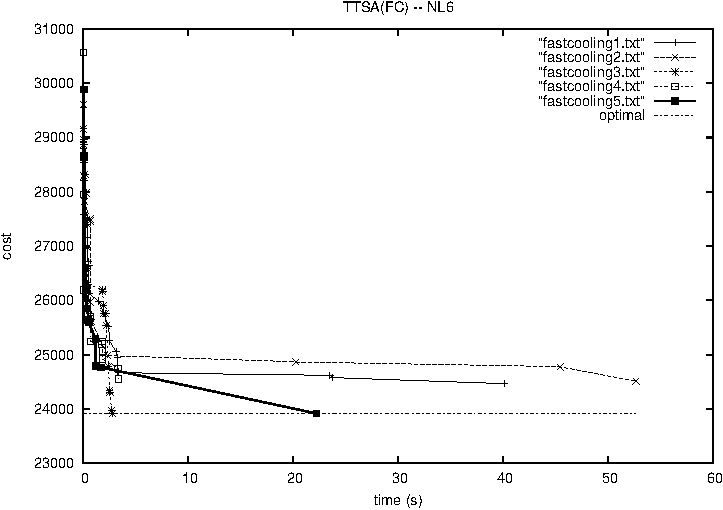
\includegraphics[width=0.75\textwidth,keepaspectratio=true]{fastcoolingNL6}
 \caption{TTSA (FC) NL6.}
 \label{fig:ttsafc6}
 \end{figure}

\begin{figure}[hbpt]
\centering
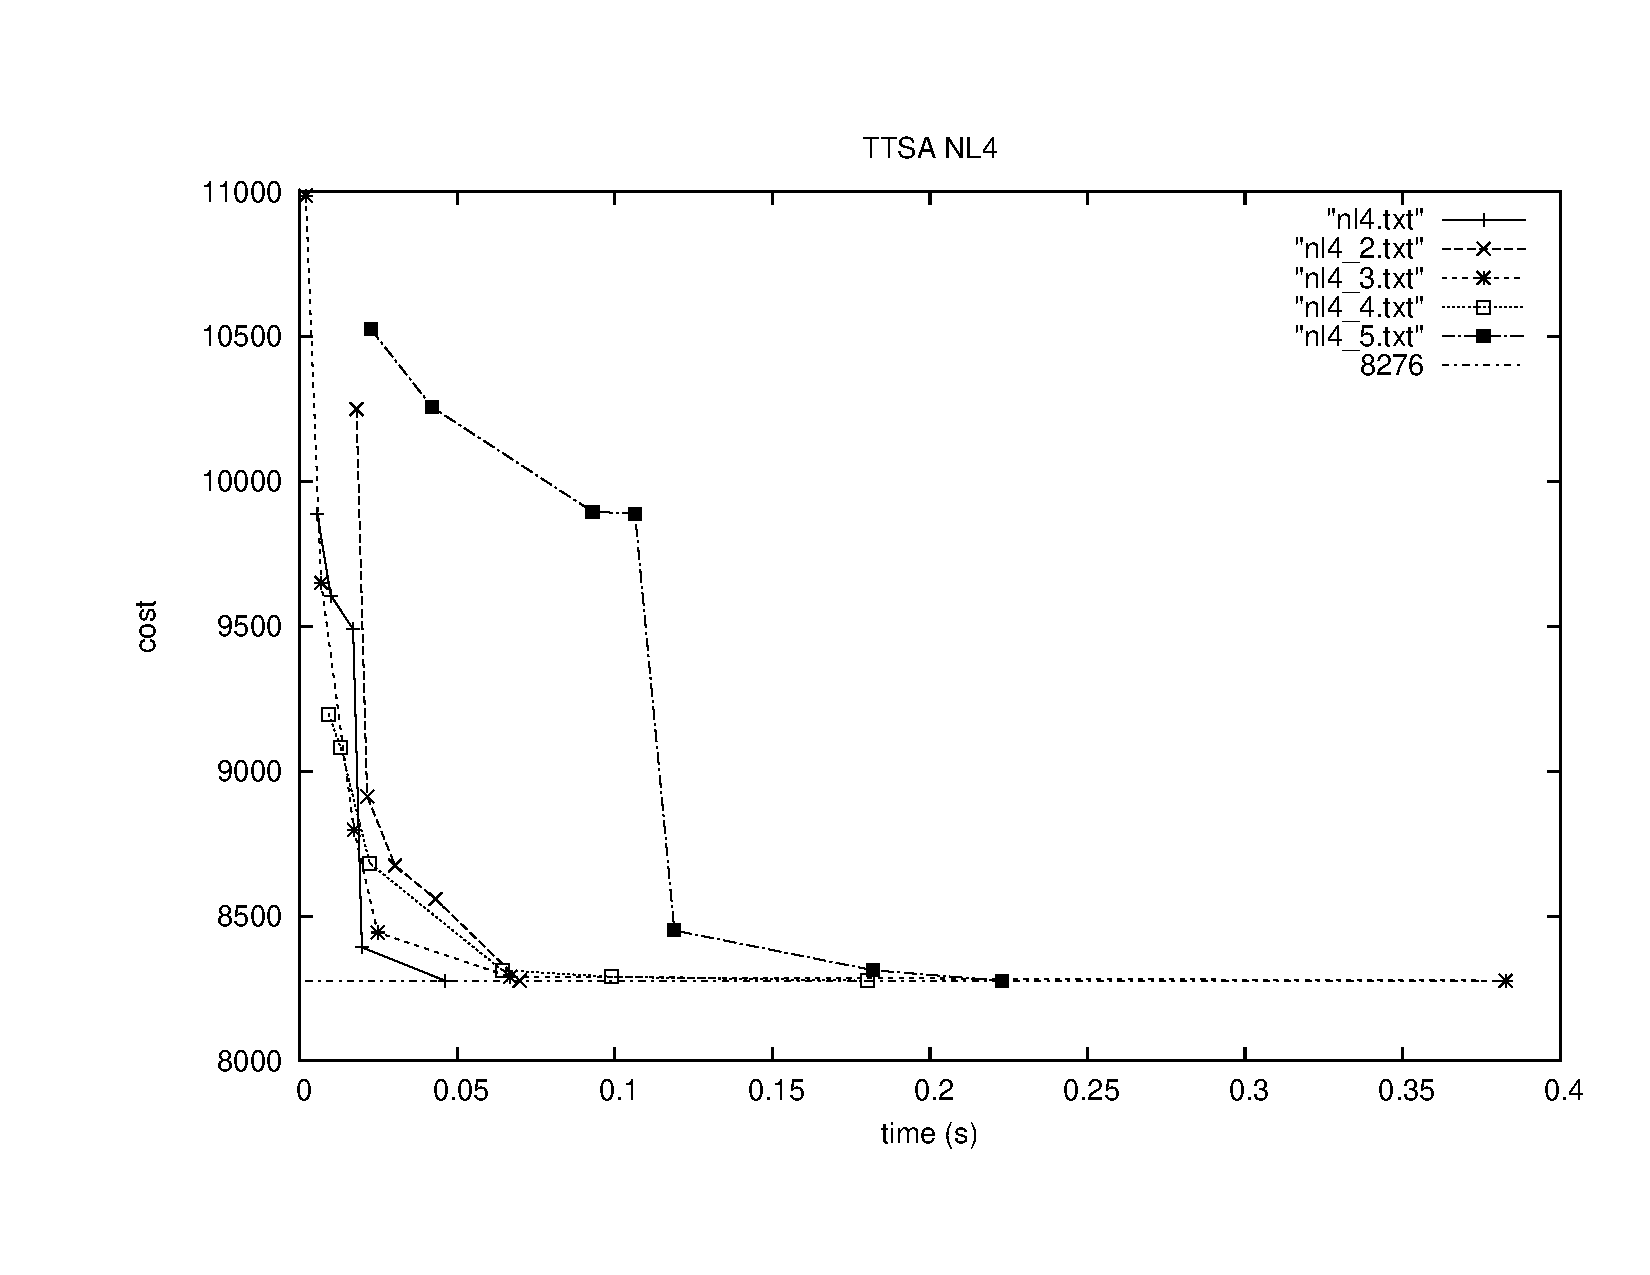
\includegraphics[width=0.75\textwidth,keepaspectratio=true]{ttsaNL4}
 \caption{TTSA NL4.}
 \label{fig:nl4}
 \end{figure}

Het probleem NL4 is triviaal: optimale oplossingen worden in enkele seconden gevonden en de parameters hebben hierbij heel weinig invloed (figuur~\ref{fig:nl4}). Voor NL6 en NL8 werden de optimale oplossingen gevonden; voor NL8 gebeurde dit echter slechts eenmaal en hebben we niet verder geprobeerd wegens tijdsoverwegingen (figuur~\ref{fig:nl8}).

\begin{figure}[hbpt]
\centering
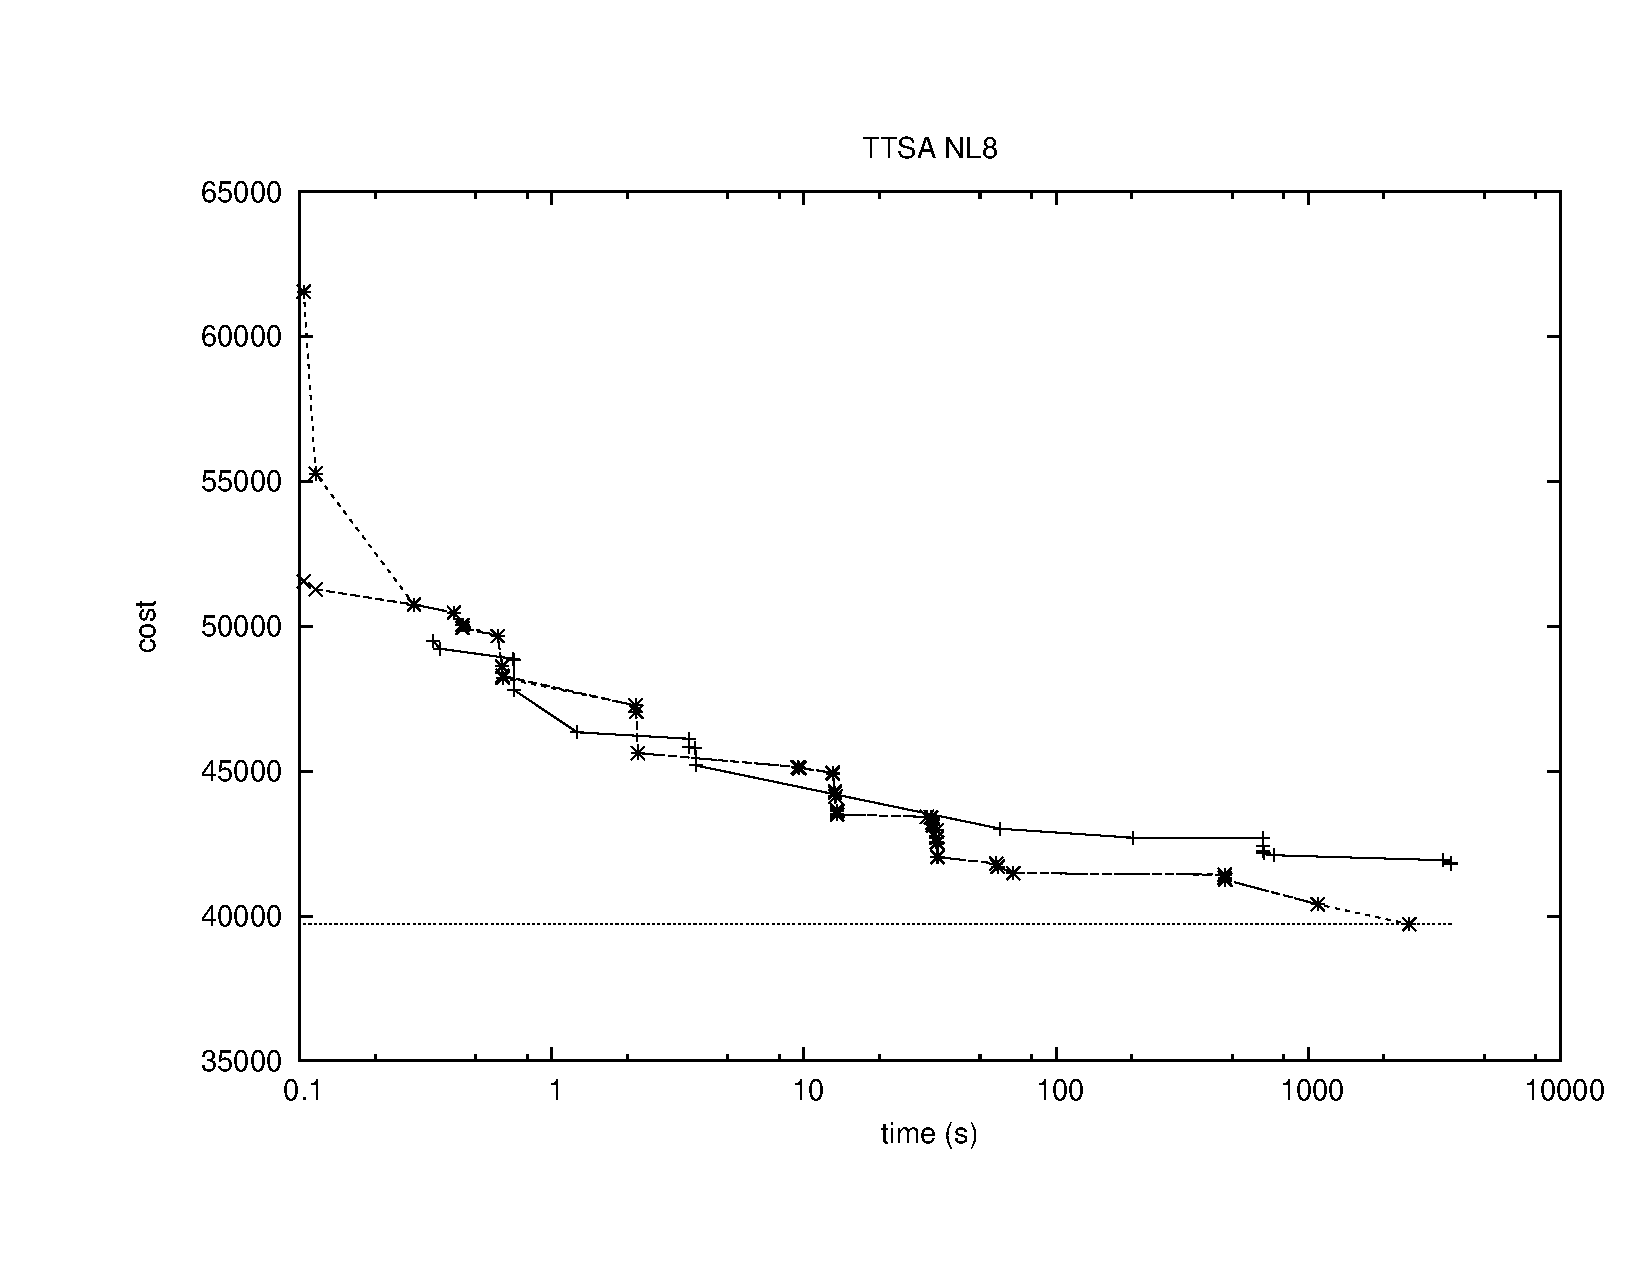
\includegraphics[width=0.8\textwidth,keepaspectratio=true]{ttsaNL8}
 \caption{TTSA NL8.}
 \label{fig:nl8}
 \end{figure}

Figuur~\ref{fig:nl12}, \ref{fig:nl14}, \ref{fig:nl16} toont de resultaten voor respectievelijk NL12, 14 en 16 op een logaritmische tijdsas.

\begin{figure}[hbpt]
\centering
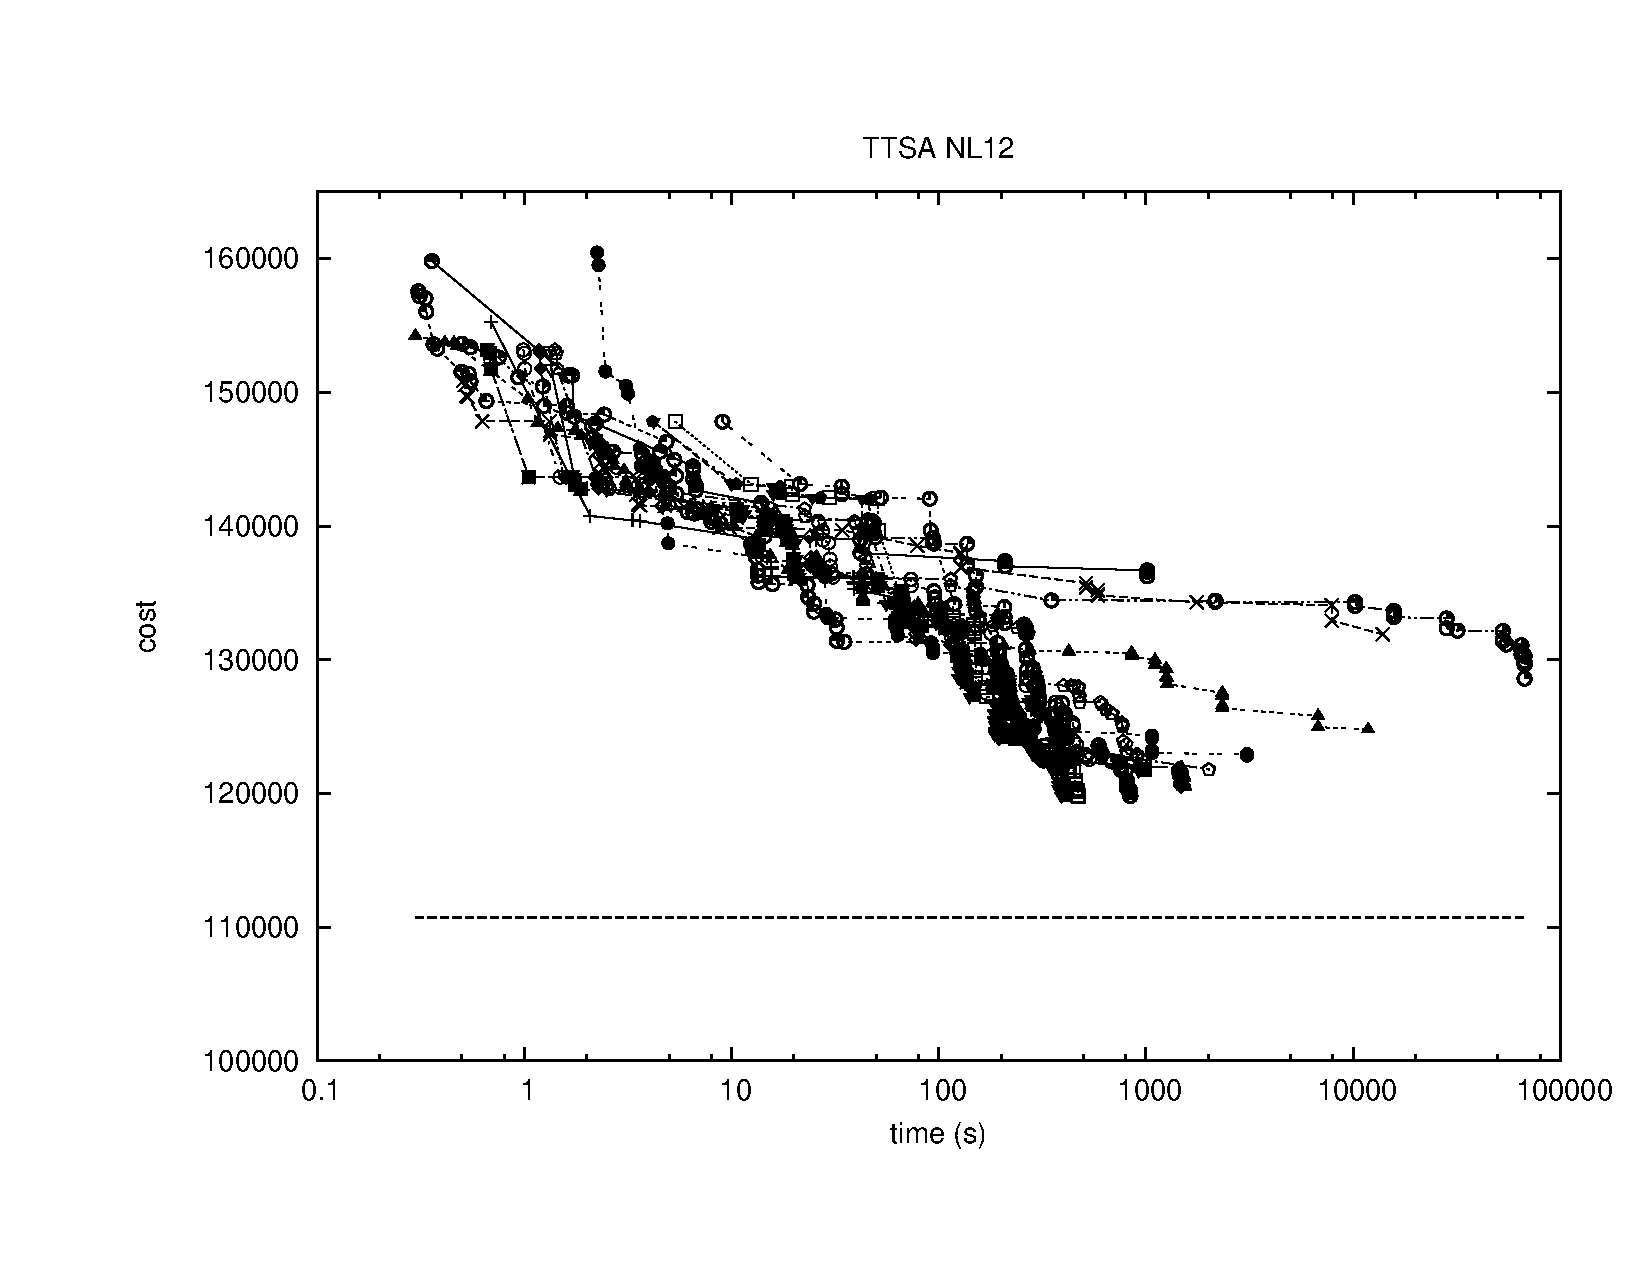
\includegraphics[width=0.8\textwidth,keepaspectratio=true]{ttsaNL12}
 \caption{TTSA NL12 (logaritmische tijdsas).}
 \label{fig:nl12}
 \end{figure}

\begin{figure}[hbpt]
\centering
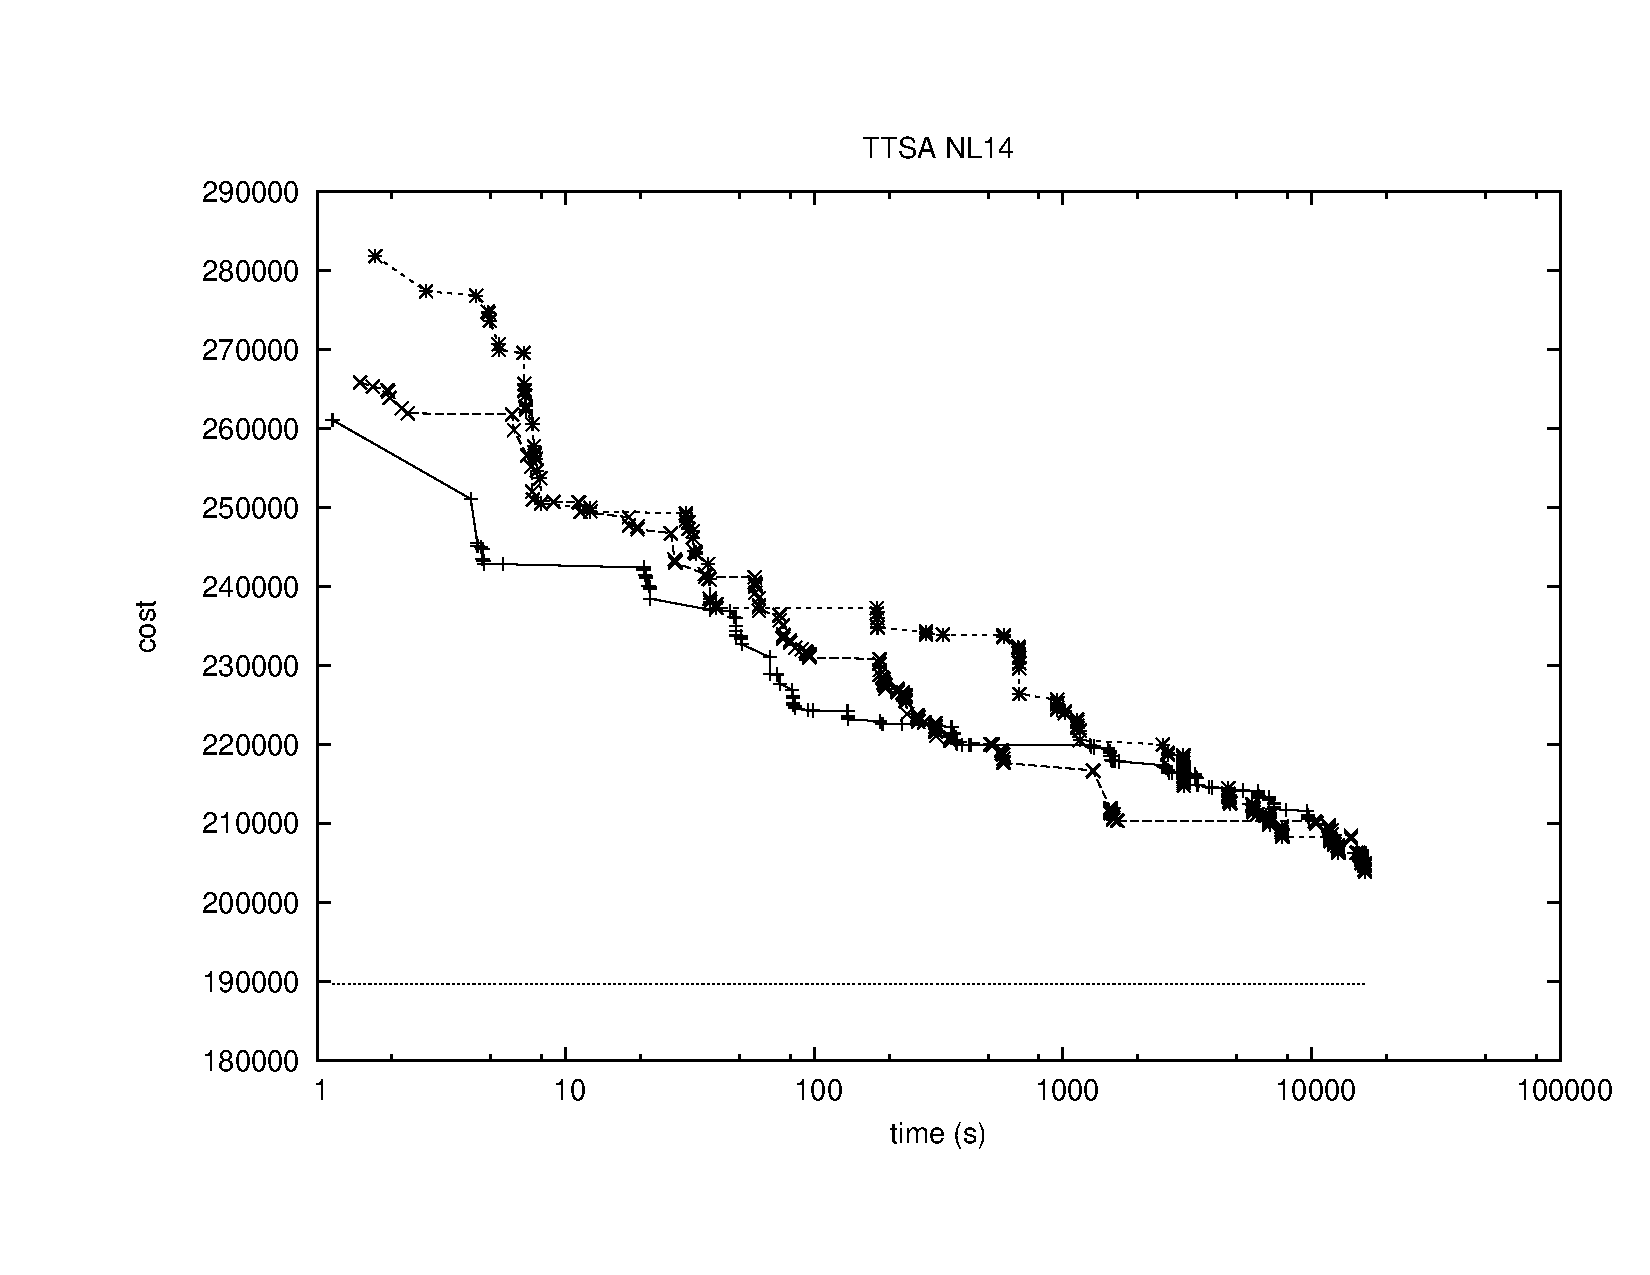
\includegraphics[width=0.8\textwidth,keepaspectratio=true]{ttsaNL14}
 \caption{TTSA NL14 (logaritmische tijdsas).}
 \label{fig:nl14}
 \end{figure}

\begin{figure}[hbpt]
\centering
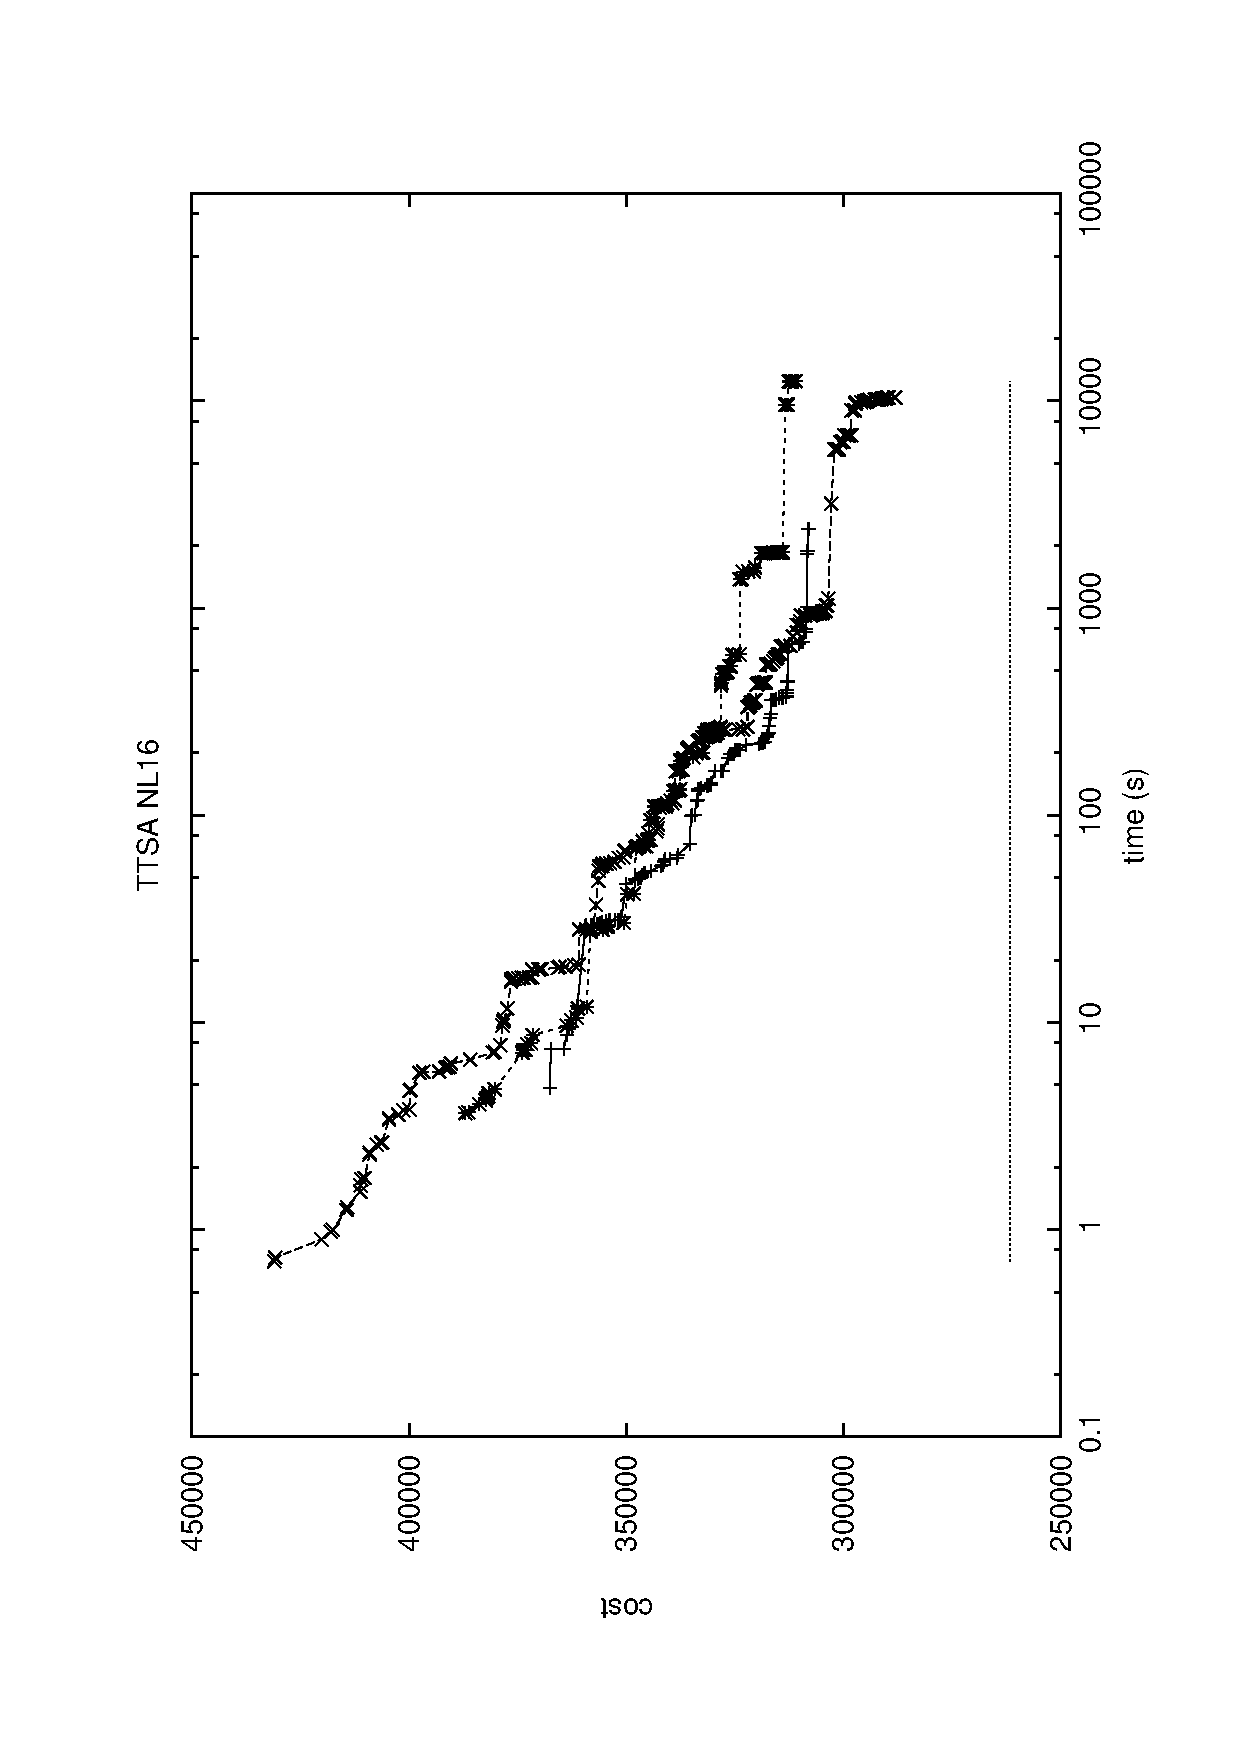
\includegraphics[width=0.8\textwidth,keepaspectratio=true]{ttsaNL16}
 \caption{TTSA NL16 (logaritmische tijdsas).}
 \label{fig:nl16}
 \end{figure}


\begin{table}[hbpt] \centering\footnotesize
\begin{tabular}
{ c   r      S  r    *{3}{S}    r  r          r           r  } \toprule
{$n$} & {cost} & {time (s)} & {$T_0$} & {$\beta$} & {$\delta$} & {$\theta$} & {$maxC$} & {$maxP$} & {$maxR$} & {$w_0$} \\  \midrule

4 & 8276    &	1.2 & 500&	0.99&	1.04&	1.04&	10&	30&	1&	4000 \\
4 & 8276    &	2.2 & 500&	0.99&	1.04&	1.04&	10&	30&	1&	4000\\
4 & 8276     &   0.8 & 500&	0.99&	1.04&	1.04&	10&	30&	1&	4000\\
4 &8276    &	1.2	& 500&	0.99&   1.04&	1.04&	10&	30& 1&	4000\\
4 & 8276    &	1.1	& 500&	0.99&	1.04&	1.04&	10&	30&	1&	4000\\ \addlinespace

6 & 23916 &	225 &	400&	0.99  & 1.04&	1.04&  100 & 100 &	5 &	4000\\
6 & 23916 &	822 &	400&    0.999 &	1.04&	1.04&  5000& 7100&	10&	4000\\
6 & 23916 &	27  &	400&	0.999 &	1.04&	1.04&  100 & 100 &	10&	4000\\
6 & 23916 &	78  &	500&	0.9999&	1.04&   1.04&  50  & 100 &	1 &	4000\\
6 & 24108 & 326 &	500&	0.99  & 1.04&	1.04&  50  & 100 &	1 &	4000     \\
6 & 23916 & 6923&	400&	0.9999& 1.04&	1.04&  5000& 7100&	10&	4000\\
6 & 24070&	371	&400&	0.99&	1.04&	1.04&	100	&100&	3&  4000  \\
6 & 23916&  184	&400&	0.99&	1.04&	1.04&	100 &50 &	2&	4000\\
6 & 24073&	572	&400&	0.99&	1.04&   1.04&	100 &100&	3&	4000\\
6 & 24073&	616	&400&	0.99&	1.04&   1.04&	100	&100&	5&	4000\\
6 & 23916&	225	&400&	0.99&	1.04&   1.04&	100	&100&	5&	4000\\
6 & 23916&	905	&400&	0.99&	1.04&   1.04&	200	&100&	5&	4000\\ \addlinespace

8&40395&	812&	400&	0.99	&1.04	&1.04	&100	&50	&2&	4000\\
8&40340&	1102&	400&	0.99	&1.04	&1.04	&100	&100	&3&	4000\\
8&41126&	301&	400&	0.99	&1.04	&1.04	&100	&100	&1&	4000\\
8&40720&	484&	400&	0.99	&1.04	&1.04	&100	&50	&5&	4000\\
8&41838&	141&	400&	0.99	&1.04	&1.04	&50	&50	&5&	4000\\
8&40228&	270&	400&	0.99	&1.04	&1.04	&50	&100	&3&	4000\\
8&39987&	645&	400&	0.99	&1.04	&1.04	&200	&50	&3&	4000\\
8&40898&	891&	400&	0.99	&1.04	&1.04	&200	&100	&1&	4000\\
8&40018&	213&	400&	0.99	&1.04	&1.04	&100	&50	&3&	4000\\
8&40952&	507&	400&	0.99	&1.04	&1.04	&150	&75	&3&	4000\\
8&39891&	12941&	500&	0.999&	1.04	&1.04	&200	&500	&2&	4000\\
8&39721&	4834&	400&	0.999&	1.04	&1.04	&4000	&7000	&10&	4000\\ \addlinespace

10&66689&	544 &	500&	0.99	&1.04	&1.04	&100	&100	&1	&4000\\
10&66562&	4760&	400&	0.999	&1.04	&1.04	&1000	&100	&7	&4000\\
10&66209&	507	&500&	0.99	&1.04	&1.04	&100	&100	&1	&4000\\
10&65088&	641	&400&	0.99	&1.04	&1.04	&100	&50	&10	&4000\\
10&64379&	414	&400&	0.99	&1.04	&1.04	&100	&50	&7	&4000\\
10&64057&	1903&400&	0.99	&1.04	&1.04	&100	&50	&5	&4000\\ 
10 & 62106 &   417 &  400 & 0.99 & 1.04 & 1.04 & 100 & 50 & 4 & 4000 \\\bottomrule
\end{tabular}
\caption{Experimenten voor NL$n$ instanties\label{tab:experimenten}.}
\end{table}


Tabel~\ref{tab:experimenten} en~\ref{tab:experimenten2} toont alle resultaten en parameters van de uitgevoerde experimenten. Merk op dat de tijd aangeduid de tijd nodig was om de oplossing gegeven in de tabel te zoeken en niet de tijd voor het eindigen van het algoritme.\footnote{Een voorbeeld hiervan is de tijd nodig voor het experiment van NL14 waarbij de oplossing in de tabel na 612\,s werd gevonden; na 6 uur werd geen betere oplossing gevonden en werd het algoritme afgebroken.}

\begin{table}[hbpt] \centering\footnotesize
\begin{tabular}
{ c   r      S  r    *{3}{S}    r  r          r           r  } \toprule
{$n$} & {cost} & {time (s)} & {$T_0$} & {$\beta$} & {$\delta$} & {$\theta$} & {$maxC$} & {$maxP$} & {$maxR$} & {$w_0$} \\  \midrule
12&125684	&15318	&500	&0.99	&1.04	&1.04	&200	&500	&1	&4000\\
12&123701	&4069	&400	&0.99	&1.04	&1.04	&100	&50	&7	&4000\\
12&127697	&1171	&400	&0.99	&1.04	&1.04	&100	&50	&7	&10000\\
12&126360	&3663	&400	&0.9	&1.04	&1.04	&100	&50	&5	&10000\\
12 & 125583    & 65 & 700 & 0.99 & 1.04 & 1.04 & 200 & 100 & 4 & 4000 \\
12 & 121750 & 2606 & 500 & 0.99 & 1.04 & 1.04 & 200 & 100 & 5 & 4000\\
12 & 119807 & 3197 & 500 & 0.99 & 1.04 & 1.04 & 200 & 100 & 5 & 4000\\
12 & 119257 & 4479 & 500 & 0.99 & 1.04 & 1.04 & 200 & 100 & 5 & 4000\\
12 & 118499 & 7450 & 500 & 0.99 & 1.04 & 1.04 & 200 & 100 & 5 & 4000\\
12 & 121750 & 946 & 500 & 0.99 & 1.04 & 1.04 & 200 & 100 & 5 & 4000\\
12 & 121750 & 2618 & 500 & 0.99 & 1.04 & 1.04 & 200 & 100 & 5 & 4000\\
12 & 119807 & 472 & 500 & 0.99 & 1.04 & 1.04 & 200 & 100 & 5 & 4000\\
12 & 120526 & 1524 & 500 & 0.99 & 1.04 & 1.04 & 200 & 100 & 5 & 4000\\
12 & 121750 & 924 & 500 & 0.99 & 1.04 & 1.04 & 200 & 100 & 5 & 4000\\
12 & 119807 & 392 & 500 & 0.99 & 1.04 & 1.04 & 200 & 100 & 5 & 4000\\
12 & 120526 & 1479 & 500 & 0.99 & 1.04 & 1.04 & 200 & 100 & 5 & 4000\\
12 & 121750 & 928 & 500 & 0.99 & 1.04 & 1.04 & 200 & 100 & 5 & 4000\\
12 & 121750 & 2015 & 500 & 0.99 & 1.04 & 1.04 & 200 & 100 & 5 & 4000\\
12 & 119807 & 421 & 500 & 0.99 & 1.04 & 1.04 & 200 & 100 & 5 & 4000\\
12 & 119807 & 844 & 500 & 0.99 & 1.04 & 1.04 & 200 & 100 & 5 & 4000\\
12 & 121750 & 1288 & 500 & 0.99 & 1.04 & 1.04 & 200 & 100 & 5 & 4000\\
12 & 121043 & 1516 & 500 & 0.99 & 1.04 & 1.04 & 200 & 100 & 5 & 4000\\
12 & 120084 & 2850 & 500 & 0.99 & 1.04 & 1.04 & 200 & 100 & 5 & 4000\\ \addlinespace

14 & 217159 &	612 &	500 &	0.999 &	1.04 &	1.04 & 	500 &	100 &	1	& 5000 \\
14 & 210680 &	9727 &	500 &	0.99 &	1.04 &	1.04 & 	200 &	100 &	5	& 4000 \\
14 & 208091 &	14408 &	500 &	0.99 &	1.04 &	1.04 & 	200 &	100 &	5	& 4000 \\
14 & 203979 &	16406 &	600 &	0.99 &	1.03 &	1.03 & 	3000 &	1500 &	10	& 10000 \\ \addlinespace

16& 302671	&5068&	400&	0.99&	1.04&	1.04&	100	&100&	2&	4000\\
16& 288089	&10392	&400&	0.9999&	1.04&	1.04&	10000&	7100&	50&	60000\\\bottomrule
\end{tabular}
\caption{Experimenten voor NL$n$ instanties (\emph{vervolg})\label{tab:experimenten2}.}
\end{table}


 
Tabel~\ref{best} vat de beste gevonden resultaten samen en vergelijkt deze met enerzijds de beste in de paper en anderzijds de beste (gepubliceerde) resultaten op~\cite{website} van 2002 en 2010. Voor de kleinere instanties werden de optimale oplossingen gevonden (die reeds bekend waren). Voor NL12 werd een betere oplossing gevonden dan de best gekende in 2002; onze oplossing is echter nog steeds slechter dan die van de auteurs.
